\chapter{Amortized optimization foundations}
\label{sec:foundations}

\begin{figure}[ht!]
  \centering
  \resizebox{\textwidth}{!}{
  \begin{tikzpicture}[every node/.style={align=left,anchor=west}]
    \node[align=right,text width=2.4in] at (0.,0.) (model) {Amortization model $\hat y_\theta$ (\cref{sec:model})};
    \node[right=.4in of model,yshift=2.5mm,text width=3.5in] (full) {Fully-amortized (\cref{sec:model:full}): no objective access};
    \node[below=-1mm of full,text width=3.5in] (semi) {Semi-amortized (\cref{sec:model:semi}): accesses objective};
    \node[below=.4in of model,align=right,text width=2.4in] (loss) {Amortization loss $\gL$ (\cref{sec:learning})};
    \node[right=.4in of loss,yshift=2.5mm,text width=3.5in] (regression) {Regression (\cref{sec:learning:reg}): $\E_{p(x)} \|\hat y_\theta(x)-x\|_2^2$};
    \node[below=-1mm of regression,text width=3.5in] (objective) {Objective (\cref{sec:learning:grad}): $\E_{p(x)} f(\hat y_\theta(x))$};
    \draw[->] (model.east) -- (full.west);
    \draw[->] (model.east) -- (semi.west);
    \draw[->] (loss.east) -- (regression.west);
    \draw[->] (loss.east) -- (objective.west);
  \end{tikzpicture}}
  \label{fig:foundations}
  \caption{Overview of amortized optimization modeling and loss choices.}
\end{figure}


The machine learning, statistics, and optimization
communities are exploring methods of \emph{learning
to optimize} to obtain fast solvers for \cref{eq:opt}.
I will refer to these methods as \emph{amortized optimization}
as they \emph{amortize} the cost of solving the
optimization problems across many contexts to approximate
the solution mapping $y^\star$.
Amortized optimization is promising because in many applications,
there are significant correlations and structure between the
solutions which show up in $y^\star$ that a model can learn.
This tutorial follows \citet{shu2017amortized} for defining the core
foundation of amortized optimization.

\begin{definition}
  An \emph{amortized optimization method} to solve \cref{eq:opt}
  can be represented by
  $\gA\defeq (f, \gY, \gX, p(x), \hat y_\theta, \gL)$,
  where
  $f: \gY\times\gX \rightarrow \R$ is the
  unconstrained \emph{objective} to optimize,
  $\gY$ is the \emph{domain},
  $\gX$ is the \emph{context space},
  $p(x)$ is the \emph{probability distribution over contexts} to optimize,
  $\hat y_\theta: \gX\rightarrow \gY$ is the \emph{amortization model}
  parameterized by $\theta$
  which is learned by optimizing a \emph{loss}
  defined on all the components
  $\gL(f, \gY, \gX, p(x), \hat y_\theta)$.
  \label{def:amor}
\end{definition}

The objective $f$ and domain $\gY$ arise from
the problem setting along with the context space
$\gX$ and distribution over it $p(x)$, and
the remaining definitions of the model
$\hat y_\theta$ and loss $\gL$ are application-specific
design decisions that \cref{sec:model,sec:learning}
opens up.
These sections present the modeling and loss foundations
for the core problem in \cref{def:amor} agnostic
of specific downstream applications that will use them.
The key choices highlighted in \cref{fig:foundations}
are how much information
1) the model $\hat y_\theta$ has about the
objective $f$ (fully- vs.~semi-amortized), and
2) the loss has about the true solution $y^\star$
(regression- vs.~objective-based).
\Cref{fig:overview} instantiates these components
for amortizing the control of a robotic system.
The model $\hat y_\theta$ solves the solution mapping
$y^\star$ simultaneously for all contexts.
The methods here usually assume the solution mapping
$y^\star$ to be almost-everywhere smooth
and well-behaved.
The best modeling approach is an open research topic
as there are many tradeoffs,
and many specialized insights from the application domain
can significantly improve the performance.
The generalization capacity along with the model's
convergence guarantees are challenging topics
which \cref{sec:generalization} covers in more detail.

\textbf{Origins of the term ``amortization'' for optimization.}
The word ``amortization'' generally means to spread out costs and
thus ``amortized optimization'' usually means to spread out
computational costs of the optimization process.
The term originated in the variational inference community
for inference optimization
\citep{kingma2013auto,rezende2014stochastic,stuhlmuller2013learning,gershman2014amortized,webb2017faithful,ravi2018amortized,cremer2018inference,wu2020meta},
and is used more generally in
\citet{xue2020amortized,sercu2021neural,xiao2021amortized}.
\citet[p.~28]{marino2021learned} give further background on the
origins and uses of amortization.
Concurrent to these developments, other communities have
independently amortization methods without referring to them
by the same terminology and analysis, such as in reinforcement learning,
policy optimization, and sparse coding ---
\cref{sec:apps} connects all of these under \cref{def:amor}.

\textbf{Conventions and notation.}
The context space $\gX$ represents the
sample space of a probability space that
the distribution $p(x)$ is defined on,
assuming it is Borel if not otherwise specified.
For a function $f: \R^n\rightarrow\R$ in standard Euclidean space,
$\nabla_x f(\bar x)\in \R^n$ denotes the \emph{gradient} at a point $\bar x$
and $\nabla^2_x f(\bar x)\in\R^{n\times n}$ denotes the \emph{Hessian}.
For $f: \R^n\rightarrow\R^m$, $\D_x f(\bar x)\in\R^{m\times n}$
represents the \emph{Jacobian} at $\bar x$ with
entries $[\D_x f(\bar x)]_{ij}\defeq \frac{\partial f_i}{\partial x_j}(\bar x)$.
I abbreviate the loss to $\gL(\hat y_\theta)$
when the other components can be inferred from the
surrounding text and prefer the term ``context'' for $x$ instead of
``parameterization'' to make the distinction between the
$x$-parameterized optimization problem
and the $\theta$-parameterized model clear.
I use ``;'' as separation in $f(y; x)$ to emphasize the separation
between the domain variables $y$ that \cref{eq:opt}
optimizes over from the context ones $x$ that remain fixed.
A model's parameters $\theta$ are usually subscripts
as $h_\theta(x)$ but I will equivalently write
$h(x; \theta)$ sometimes.

\section{Defining the model $\hat y_\theta(x)$}
\label{sec:model}
The model $\hat y_\theta(x): \gX\times\Theta\rightarrow \gY$
predicts a solution to \cref{eq:opt}.
In many applications, the best model design is an active
area of research that is searching for models that are
expressive and more computationally efficient than the
algorithms classically used to solve the optimization problem.
\Cref{sec:model:full} starts simple with \emph{fully-amortized} models
that approximate the entire solution
to the optimization problem with a single black-box model.
Then \cref{sec:model:semi} shows how to open up the model
to include more information about the optimization problem
that can leverage domain knowledge with \emph{semi-amortized} models.

\subsection{Fully-amortized models}
\label{sec:model:full}
\begin{definition}
  A \emph{fully-amortized} model $\hat y_\theta: \gX\rightarrow\gY$
  maps the context to the solution of \cref{eq:opt}
  and does \emph{not} access the objective $f$.
\end{definition}

I use the prefix ``fully'' to emphasize
that the entire computation of the solution to the
optimization problem is absorbed into
a black-box model that does \emph{not} access the objective $f$.
The prefix ``fully'' can be omitted when the context is clear
because most amortization is fully amortized.
These are standard in amortized variational inference
(\cref{sec:apps:avi}) and policy
leaning (\cref{sec:apps:ctrl}), that typically use
feedforward neural networks to map from
the context space $\gX$ to the solution of the
optimization problem living in $\gY$.
Fully-amortized models are remarkable because they
are often successfully able to predict the solution
to the optimization problem in \cref{eq:opt}
\emph{without} ever accessing the objective of
the optimization problem after being trained.

Fully-amortized models are the most useful for attaining approximate
solutions that are computationally efficient.
They tend to work the best when the
solution mappings $y^\star(x)$ are predictable,
the domain $\gY$ is relatively small,
usually hundreds or thousands of dimensions,
and the context distribution isn't too large.
When fully-amortized models don't work well,
semi-amortized models help open up the black box
and use information about the objective.

\subsection{Semi-amortized models}
\label{sec:model:semi}
\begin{definition}
  A \emph{semi-amortized} model $\hat y_\theta: \gX\rightarrow\gY$
  maps the context to the solution of the optimization problem
  and accesses the objective $f$ of \cref{eq:opt},
  typically iteratively.
\end{definition}

\citet{kim2018semi,marino2018iterative}
proposed \emph{semi-amortized} models for variational inference
that add back domain knowledge of the optimization problem
to the model $\hat y_\theta$ that the fully-amortized
models do not use.
These are brilliant ways of integrating the optimization-based
domain knowledge into the learning process.
The model can now internally integrate
solvers to improve the prediction.
Semi-amortized methods are typically iterative and update
iterates in the domain $\gY$ or in an \emph{auxiliary}
or \emph{latent space} $\gZ$.
I refer to the space the semi-amortization iterates over
as the \emph{amortization space} and denote iterate $t$
in these spaces, respectively, as $\hat y^{t}_\theta$ and $z^t_\theta$.
While the iterates and final prediction $\hat y_\theta$
can now query the objective $f$ and gradient $\nabla_y f$,
I notationally leave this dependence implicit for
brevity and only reference these queries in the relevant definitions.

\subsubsection{Semi-amortized models over the domain $\gY$}
\label{sec:semi-domain}
\begin{center}
\begin{tikzpicture}
  \matrix (m) [
      matrix of math nodes,row sep=2em,column sep=1em,
      minimum width=2em,nodes={anchor=center}
  ] {
    \hat y^{0}_\theta & \hat y_\theta^{1} &
    \ldots & \hat y_\theta^{K}\eqdef \hat y_\theta(x) \\
  };
  \path[-stealth]
    (m-1-1) edge node {} (m-1-2)
    (m-1-2) edge node {} (m-1-3)
    (m-1-3) edge node {} (m-1-4);
\end{tikzpicture}
\end{center}
\vspace{-3mm}

One of the most common semi-amortized model is to
parameterize and integrate an optimization procedure
used to solve \cref{eq:opt} into the model $\hat y_\theta$,
such as gradient descent \citep{andrychowicz2016learning,finn2017model,kim2018semi}.
This optimization procedure is an internal part of
the amortization model $\hat y_\theta$,
often referred to as the \emph{inner-level} optimization
problem in the bi-level setting that arises for learning.

\textbf{Examples.}
This section instantiates a canonical semi-amortized model based
gradient descent that learns the initialization as in
model-agnostic meta-learning (MAML) by \citet{finn2017model},
structured prediction energy networks (SPENs) by \citet{belanger2017end},
and semi-amortized variational auto-encoders (SAVAEs) by \citet{kim2018semi}.
The initial iterate $\hat y^{0}_\theta(x)\defeq \theta$
is parameterized by $\theta\in\gX$ for all contexts.
Iteratively updating $\hat y^{t}_\theta$ for $K$ gradient steps
with a \emph{learning rate} or \emph{step size} $\alpha\in\R_+$
on the objective $f(y;x)$ gives
\begin{equation}
  \hat y^{t}_\theta \defeq \hat y^{t-1}_\theta - \alpha \nabla_y f(\hat y^{t-1}_\theta; x) \qquad t\in\{1\ldots,K\},
  \label{eq:gd}
\end{equation}
where model's output is defined as
$\hat y_\theta\defeq \hat y^{K}$.

Semi-amortized models over the domain can go significantly beyond
gradient-based models and in theory, any algorithm to solve
the original optimization problem in \cref{eq:opt}
can be integrated into the model.
\Cref{sec:unrolled} further discusses the learning of
semi-amortized models by unrolling that are instantiated later:
\begin{itemize}
\item \Cref{sec:apps:lista} discusses how
\citet{gregor2010learning} integrate ISTA iterates
\citep{daubechies2004iterative,beck2009fast}
into a semi-amortized model.
\item \Cref{sec:apps:neural-fp} discusses models that integrate
fixed-point computations into semi-amortized models.
\citet{venkataraman2021neural} amortize convex cone programs by
differentiating through the splitting cone solver \citep{o2016conic}
and \citet{bai2022neural} amortize
deep equilibrium models \citep{bai2019deep,bai2020multiscale}.
\item \Cref{sec:apps:qprl} discusses RLQP by \citet{ichnowski2021accelerating}
  that uses the OSQP solver \citep{stellato2018osqp} inside
  of a semi-amortized model.
\end{itemize}

\subsubsection{Semi-amortized models over a latent space $\gZ$}
\label{sec:semi-latent}
\begin{center}
\begin{tikzpicture}
  \matrix (m) [
      matrix of math nodes,row sep=2em,column sep=1em,
      minimum width=2em,nodes={anchor=center}
  ] {
    \hat z^{0}_\theta & \hat z_\theta^{1} &
    \ldots & \hat z_\theta^{K} & \hat y_\theta(x) \\};
  \path[-stealth]
    (m-1-1) edge node {} (m-1-2)
    (m-1-2) edge node {} (m-1-3)
    (m-1-3) edge node {} (m-1-4)
    (m-1-4) edge node {} (m-1-5);
\end{tikzpicture}
\end{center}
\vspace{-3mm}

In addition to only updating iterates over the domain $\gY$,
a natural generalization is to introduce a latent space $\gZ$
that is iteratively optimized over \emph{inside} of
the amortization model.
This is usually done to give the semi-amortized model
more capacity to learn about the structure of the optimization
problems that are being solved.
The latent space can also be interpreted as a representation
of the optimal solution space.
This is useful for learning an optimizer that only searches
over the \emph{optimal} region of the solution space rather
than the entire solution space.

\textbf{Examples.}
The iterative gradient updates in \cref{eq:gd}
can be replaced with a learned update function as in
\citet{ravi2016optimization,li2016learning,andrychowicz2016learning,li2017learning}.
These model the past sequence of iterates and learn how
to best-predict the next iterate, pushing them towards optimality.
This can be done with a recurrent cell $g$ such
as an LSTM \citep{hochreiter1997long} or GRU \citep{cho2014learning}
and leads to updates of the form
\begin{equation}
  z^t_\theta, \hat y^{t}_\theta \defeq g_\theta(z^{t-1}_\theta, x^{t-1}_\theta, \nabla_y f(\hat y^{t-1}_\theta; x)) \qquad t\in\{1\ldots,K\}
  \label{eq:rec}
\end{equation}
where each call to the recurrent cell $g$
takes a hidden state $z$ along with an iterate and
the derivative of the objective.
This endows $g$ with the capacity to learn significant
updates leveraging the problem structure that a
traditional optimization method would not be able
to make.
In theory, traditional update rules can also be
fallen back on as the gradient step in \cref{eq:gd}
is captured by removing the hidden state $z$ and
setting
\begin{equation}
  g(x, \nabla_y f(y; x))\defeq x-\alpha\nabla_y f(y; x).
  \label{eq:rec-grad-step}
\end{equation}

Latent semi-amortized models are a budding topic and can
excitingly learn many other latent representations
that go beyond iterative gradient updates in the original
space.
\citet{luo2018neural,amos2019dcem}
learn a \emph{latent domain} connected to the
original domain where the latent domain captures
hidden structures and redundancies present in
the original high-dimensional domain $\gY$.
\citet{luo2018neural} consider gradient updates
in the latent domain and \citet{amos2019dcem}
show that the cross-entropy method \citep{de2005tutorial}
can be made differentiable and learned as an alternative
to gradient updates.
\citet{amos2017input} unrolls and differentiates through
the bundle method \citep{smola2007bundle} in a convex setting
as an alternative to gradient steps.
The latent optimization could also be done over a learned parameter
space as in POPLIN \citep{wang2019exploring}, which \emph{lifts}
the domain of the optimization problem \cref{eq:opt}
from $\gY$ to the parameter space of a fully-amortized neural network.
This leverages the insight that the parameter space of
over-parameterized neural networks can induce easier
non-convex optimization problems than in the original
space, which is also studied in \citet{hoyer2019neural}.

\subsubsection{Comparing semi-amortized models with warm-starting}
Semi-amortized models are conceptually similar to learning a fully-amortized model
to warm-start an existing optimization procedure that fine-tunes the solution.
The crucial difference is that semi-amortized learning often end-to-end learns
through the final prediction while warm-starting and fine-tuning only learns
the initial prediction and does not integrate the knowledge of the fine-tuning
procedure into the learning procedure.
Choosing between these is an active research topic and while this
tutorial will
mostly focus on semi-amortized models, learning a fully-amortized
warm-starting model brings promising results to some fields too,
such as \citet{zhang2019safe,baker2019learning,chen2022large}.
In variational inference, \citet[Table 2]{kim2018semi} compare semi-amortized
models (SA-VAE) to warm-starting and fine-tuning (VAE+SVI) and demonstrate
that the end-to-end learning signal is helpful.
In other words, amortization finds an initialization that is
helpful for gradient-based optimization.
\citet{arbel2021amortized} further study fully-amortized warm-started
solvers that arise in bi-level optimization problems for
hyper-parameter optimization and use the theoretical framework from
singularly perturbed systems \citep{habets2010stabilite}
to analyze properties of the approximate solutions.

\subsubsection{On second-order derivatives of the objective}
\label{sec:second-derivatives}

Training a semi-amortized model is usually more computationally
challenging than training a fully-amortized model.
This section looks at how second-order derivatives of the
objective may come up when unrolling and create a
computational bottleneck when learning a semi-amortized model.
The next derivation follows \citet[\S5]{nichol2018first}
and \citet{weng2018metalearning} and shows the model derivatives
that arise when composing a semi-amortized model with a loss.

\textbf{Starting with a single-step model.}
This section instantiates a single-step model
similar to \cref{eq:gd} that parameterizes the initial
iterate $\hat y^0_\theta(x)\defeq\theta$ and takes one gradient step:
\begin{equation}
  \hat y_\theta(x)\defeq \hat y^0_\theta(x) - \alpha \nabla_y f(\hat y^0_\theta(x); x)
  \label{eq:single-step}
\end{equation}
Interpreting $\hat y_\theta(x)$ as a model is non-standard in contrast
to other parametric models because it makes the
optimization step \emph{internally part of the model}.
Gradient-based optimization of losses with respect to the model's parameters,
such as \cref{eq:reg-loss,eq:grad-loss} requires the Jacobian of $\hat y_\theta(x)$
w.r.t.~the parameters, \ie $\D_\theta[\hat y_\theta(x)]$
(or Jacobian-vector products with it).
Because $\hat y_\theta(x)$ is an optimization step, the derivative
of the model requires differentiating through the optimization step,
which for \cref{eq:single-step} is
\begin{equation}
  \D_\theta[\hat y_\theta(x)] = I-\alpha \nabla_y^2 f(y_\theta^0(x); x)
  \label{eq:second-derivatives-single-step}
\end{equation}
and requires the Hessian of the objective.
In \citet{finn2017model}, $\nabla_y^2 f$ is the Hessian of the
model's parameters on the training loss (!) and is
compute- and memory-expensive to instantiate for large models.
In practice, the Hessian in \cref{eq:second-derivatives-single-step}
is often never explicitly instantiated as optimizing the
loss only requires Hessian-vector products.
The Hessian-vector product can be computed exactly or
estimated without fully instantiating the Hessian, similar to
how computing the derivative of a neural network with backprop
does not instantiate the intermediate Jacobians and only computes
the Jacobian-vector product.
More information about efficiently computing Hessian-vector products
is available in \citet{pearlmutter1994fast,domke2012generic}.
Jax's \href{https://github.com/google/jax/blob/27360b9/docs/notebooks/autodiff_cookbook.ipynb}{autodiff cookbook}
\citep{bradbury2020jax}
further describes efficient Hessian-vector products.
Before discussing alternatives,
the next portion derives similar results for a $K$-step model.

\textbf{Multi-step models.}
\Cref{eq:single-step} can be extended to the $K$-step setting with
\begin{equation}
\hat y_\theta^K(x)\defeq \hat y^{K-1}_\theta(x) - \alpha\nabla_y f(\hat y^{K-1}_\theta(x); x),
\end{equation}
where the base $\hat y_\theta^0(x)\defeq\theta$ as before.
Similar to \cref{eq:second-derivatives-single-step},
the derivative of a single step is
\begin{equation}
  \D_\theta[\hat y_\theta^K(x)] = \D_\theta[\hat y_\theta^{K-1}(x)]\left(I-\alpha\nabla_y^2 f(y_\theta^{K-1}(x); x)\right),
  \label{eq:second-derivatives-recurrent}
\end{equation}
and composing the derivatives down to $\hat y_\theta^0$ yields the product structure
\begin{equation}
  \D_\theta[\hat y_\theta^K(x)] = \prod_{k=0}^{K-1} \left( I-\alpha\nabla_y^2 f(y_\theta^k(x); x) \right),
  \label{eq:second-derivatives-k-steps}
\end{equation}
where $\D_\theta[\hat y_\theta^0(x)]=I$ at the base case.
Computing \cref{eq:second-derivatives-k-steps} is
now $K$ times more challenging as it requires the Hessian
$\nabla_y^2 f$ at \emph{every} iteration of the model.
While using Hessian-vector products can alleviate some
computational burden of this term, it often still requires
significantly more operations than most other derivatives.

\textbf{Computationally cheaper alternatives.}
The first-order MAML baseline in \citet{finn2017model} suggests to
simply not use the second-order terms $\nabla_y^2 f$ here,
approximating the model derivative as the identity,
\ie $\D_\theta[\hat y_\theta^K(x)]\approx I$,
and relying on only information from the outer loss
to update the parameters.
They use the intuition from \citet{goodfellow2014explaining}
that neural networks are locally linear and therefore these
second-order terms of $f$ are not too important.
They show that this approximation works well in some cases,
such as MiniImagenet \citep{ravi2016optimization}.
The MAML$++$ extension by \citet{antoniou2018train} proposes to
use first-order MAML during the early phases of training, but
to later add back this second-order information.
\citet{nichol2018first} further analyze first-order approximations
to MAML and propose another approximation called Reptile that
also doesn't use this second-order information.
These higher-order terms also come up when unrolling in the
different bi-level optimization setting for hyper-parameter optimization,
and \citet[Table 1]{lorraine2020optimizing} gives
a particularly good overview of approximations to these.
Furthermore, memory-efficient methods for training neural networks
and recurrent models with backpropagation and
unrolling such as \citet{gruslys2016memory,chen2016training}
can also help improve the memory utilization in amortization models.

\textbf{Parameterizing and learning the objective.}
While this section has mostly not considered the setting when
the objective $f$ is also learned,
the second-order derivatives appearing in
\cref{eq:second-derivatives-k-steps}
also cause issues in when the objective is parameterized
and learned.
In addition to learning an initial iterate, \citet{belanger2017end}
learn the objective $f$ representing an energy function.
They parameterize $f$ as a neural network and use softplus
activation functions rather than ReLUs to ensure the
objective's second-order derivatives are non-zero.

\subsection{Models based on differentiable optimization}
As discussed in \cref{sec:learning}, the model typically needs
to be (sub-)differentiable with respect to the parameters
to attain the Jacobian $\D_\theta[\hat y_\theta]$
(or compute Jacobian-vector products with it)
necessary to optimize the loss.
These derivatives are standard backprop when the model
is, for example, a full-amortized neural network, but
in the semi-amortized case, the model itself is often an
optimization process that needs to be differentiated through.
When the model updates are objective-based as in
\cref{eq:gd} and \cref{eq:rec}, the derivatives with respect
to $\theta$ through the sequence of gradient updates
in the domain can be attained by seeing the updates
as a sequence of computations that are differentiated through,
resulting in second-order derivatives.
When more general optimization methods are used for
the amortization model that may not have a closed-form
solution, the tools of differentiable optimization
\citep{domke2012generic,gould2016differentiating,amos2017optnet,amos2019differentiable,agrawal2019differentiable}
enable end-to-end learning.

\subsection{Practically choosing a model}
This section has taxonomized how to instantiate an amortization
model in an application-agnostic way. As in most machine learning
settings in practice, the modeling choice is often
application-specific and needs to take into consideration many factors.
This may include 1) the speed and expressibility of the model,
2) adapting the model to specific context space $\gX$.
An MLP may be good for fixed-dimensional
real-valued spaces but a convolutional neural network
is likely to perform better for image-based spaces.
3) taking the solution space $\gY$ into consideration.
For example, if the solution space is an image space,
then a standard vision model capable of predicting
high-dimensional images is reasonable, such as a
U-net \citep{ronneberger2015u},
dilated convolutional network \citep{yu2015multi}
or fully convolutional network \citep{long2015fully}.
4) the model also may need to adapt to a
\emph{variable-length} context or solution space.
This arises in VeLO \citep{metz2022velo} for learning
to optimize machine learning models where the model needs
to predict the parameters of different models that may
have different numbers of parameters.
Their solution is to decompose the structure of the
parameter space and to formulate the semi-amortized
model as a sequence model that predicts smaller MLPs
that operate on smaller groups of parameters.

\section{Learning the model's parameters $\theta$}
\label{sec:learning}

\begin{figure}[t]
  \centering
  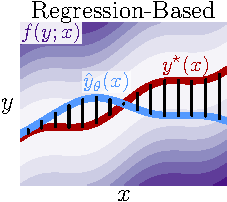
\includegraphics[width=0.32\textwidth]{fig/learning-reg.pdf}
  \hspace{10mm}
  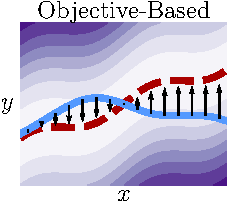
\includegraphics[width=0.32\textwidth]{fig/learning-obj.pdf}
  \caption{Overview of key losses for optimizing
    the parameters $\theta$ of the amortization model $\hat y_\theta$.
    Regression-based losses optimize a distance between
    the model's prediction $\hat y_\theta(x)$ and the
    ground-truth $y^\star(x)$. Objective-based
    methods update $\hat y_\theta$ using
    local information of the objective $f$
    and \emph{without} access to the ground-truth
    solutions $y^\star$.
  }
  \label{fig:learning}
\end{figure}

After specifying the amortization model $\hat y_\theta$, the other major
design choice is how to learn the parameters $\theta$
so that the model best-solves \cref{eq:opt}.
Learning is often a \emph{bi-level} optimization problem
where the \emph{outer level} is the parameter
learning problem for a model $\hat y_\theta(x)$ that solves
the \emph{inner-level} optimization problem in \cref{eq:opt}
over the domain $\gY$.
While defining the best loss is application-specific,
most approaches can be roughly categorized as
1) regressing a ground-truth solution (\cref{sec:learning:reg}),
or 2) minimizing the objective (\cref{sec:learning:grad,sec:learning:rl}),
which \cref{fig:learning} illustrates.
Optimizing the model parameters here can in theory be done
with most parameter learning methods that incorporate
zeroth-, first-, and higher-order information
about the loss being optimized, and this section mostly focuses
on methods where $\theta$ is learned with a
first-order gradient-based method
such as \citet{nesterov1983method,duchi2011adaptive,zeiler2012adadelta,kingma2014adam}.
The rest of this section discusses approaches for
designing the loss and optimizing the parameters
with first-order methods
(\cref{sec:learning:reg,sec:learning:grad})
when differentiation is easy
or zeroth-order methods (\cref{sec:learning:rl})
otherwise, \eg, in non-differentiable settings.

\subsection{Choosing the objective for learning}
\subsubsection{Regression-based learning}
\label{sec:learning:reg}
Learning can be done by regressing the
model's prediction $\hat y_\theta(x)$ onto a
ground-truth solution $y^\star(x)$.
These minimize some distance between the predictions
and ground-truth so that the expectation over
the context distribution $p(x)$ is minimal.
With a Euclidean distance, for example,
regression-based learning solves
\begin{equation}
  \argmin_\theta \gL_{\rm reg}(\hat y_\theta) \qquad
  \gL_{\rm reg}(\hat y_\theta) \defeq
  \E_{x \sim p(x)} \|y^\star(x) - \hat y_\theta(x) \|_2^2.
\label{eq:reg-loss}
\end{equation}
$\gL_{\rm reg}$ is typically optimized with an adaptive first-order
gradient-based method that is able to directly differentiate
the loss with respect to the model's parameters.

Regression-based learning works the best for distilling
known solutions into a faster model that can be deployed
at a much lower cost, but can otherwise start failing to work.
In RL and control, regression-based amortization
methods are referred to as \emph{behavioral cloning} and
is a widely-used way of recovering a policy using
trajectories observed from an expert policy.
Using regression is also advantageous when evaluating
the objective $f(y;x)$ incurs a computationally intensive
or otherwise complex procedure, such as an evaluation of
the environment and dynamics in RL, or for
computing the base model gradients when learning parameter optimizers.
These methods work well when the ground-truth solutions
are unique and semi-tractable, but can fail otherwise,
\ie if there are many possible ground-truth
solutions for a context $x$ or if computing them
is too intractable.
After all, solving \cref{eq:opt} from scratch may be
computationally expensive and amortization methods
should improve the computation time.

\begin{remark}
  \Cref{eq:reg-loss} can be extended to other distances
  defined on the domain, such as non-Euclidean distances
  or the likelihood of a probabilistic model that predicts
  a distribution of possible candidate solutions.
  \citet{adler2017learning} propose to use the Wasserstein
  distance for learning to predict the solutions to
  inverse imaging problems.
\end{remark}

\subsubsection{Objective-based learning}
\label{sec:learning:grad}

Instead of regressing onto the ground-truth solution,
\emph{objective-based} learning methods seek for
the model's prediction to be minimal under the objective $f$ with:
\begin{equation}
  \argmin_\theta \gL_{\rm obj}(\hat y_\theta) \qquad \gL_{\rm obj}(\hat y_\theta) \defeq \E_{x \sim p(x)} f(\hat y_\theta(x); x).
\label{eq:grad-loss}
\end{equation}
These methods use local information of the objective
to provide a descent direction for the model's
parameters $\theta$.
A first-order method optimizing \cref{eq:grad-loss} uses
updates based on the gradient
\begin{equation}
  \begin{aligned}
  \nabla_\theta \gL_{\rm obj}(\hat y_\theta) &= \nabla_\theta \left[ \E_{x\sim p(x)}f(\hat y_\theta(x); x)\right] \\
  &= \E_{x\sim p(x)} \D_\theta\left[ \hat y_\theta(x)\right]^\top
  \nabla_{y} \left[ f(\hat y_\theta(x); x) \right],
  \end{aligned}
  \label{eq:grad-loss-grad}
\end{equation}
where the last step is obtained by the chain rule.
This has the interpretation that the model's parameters $\theta$
are updated by combining the gradient information around the prediction
$\nabla_{y} \left[ f(\hat y_\theta(x); x) \right]$
shown in \cref{fig:learning} along with
how $\theta$ impacts the model's predictions with the derivative
$\D_\theta\left[ \hat y_\theta(x)\right]$.
While this tutorial mostly focuses on optimizing
\cref{eq:grad-loss-grad} with
first-order methods that explicitly differentiate
the objective, \cref{sec:learning:rl} discusses alternatives
to optimizing it with reinforcement learning and
zeroth-order methods.

Objective-based methods thrive when the gradient information
is informative and the objective and models are easily differentiable.
Amortized variational inference methods and
actor-critic methods both make extensive use of
objective-based learning.

\begin{remark}
  A standard gradient-based optimizer for \cref{eq:opt} (without amortization)
  can be recovered from $\gL_{\rm obj}$ by setting the model to the identity
  of the parameters, \ie $\hat y_\theta(x)\defeq\theta$, and $p(x)$ to be a
  Dirac delta distribution.
  \label{remark:obj-loss}
\end{remark}

This can be seen by taking $\D_\theta[\hat y_\theta(x)]=I$
in \cref{eq:grad-loss-grad}, resulting in
$\nabla_\theta \gL_{\rm obj}(\hat y_\theta)=\nabla_y f(\hat y_\theta(x); x)$.
Thus optimizing $\theta$ of this parameter-identity model with gradient descent
is identical to solving \cref{eq:opt} with gradient descent.
\Cref{remark:obj-loss} shows a connection between a model trained with
gradients of an objective-based loss and a non-amortized gradient-based
solver for \cref{eq:opt}.
The gradient update that would originally have been applied to an
iterate $y\in\gY$ of the domain is now transferred into the
model's parameters that are shared across all problem instances.
This also leads to a hypothesis that objective-based amortization
works best when a gradient-based optimizer is able to successfully
solve \cref{eq:opt} from scratch. However there may be settings
where a gradient-based optimizer performs poorly but an amortized
optimizer excels because it is able to use information from the
other problem instances.

\begin{remark}
The objective-based loss in \cref{sec:learning:grad} provides a starting
point for amortizing with other optimality conditions or reformulations
of the optimization problem. This is done when amortizing for fixed-point
computations and convex optimization in \cref{sec:apps:convex}, as well as
in optimal transport \cref{sec:apps:ot}.
\label{rmk:optimality-loss}
\end{remark}

\subsubsection{Comparing the regression- and objective-based losses}
\begin{figure}[t]
\centering
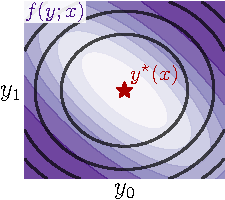
\includegraphics[width=2in]{fig/loss-comp.pdf}
\caption{Contours of the regression-based amortization loss
  $\gL_{\rm reg}$ (in black) alongside the contours of the objective
  (in purple where darker colors indicate higher values).
  This shows the inaccuracies of the regression-based loss, \eg
  along a level set, may impact the overall objective differently.
}
\label{fig:reg-contours}
\end{figure}

Choosing between the regression- and objective-based losses
is challenging as they measure the solution quality in
different ways and have different convergence and
locality properties.
\citet{liu2022teaching} experimentally compare these
losses for learning to optimize with fully-amortized set-based models.
\Cref{fig:reg-contours} illustrates that the $\ell_2$-regression
loss (the black contours) ignores the objective
values (the purple contours) and thus gives the same loss
to solutions that result in significantly different
objective values.
This could be potentially addressed by normalizing or
re-weighting the dimensions for regression to be more aware
of the curvature of the objective, but this is often not done.
Another idea is to combine both the objective and regression losses.
Combining the losses could work especially well when only a
few contexts are labeled, such as the regression and residual terms
in the physics-informed neural operator paper \citep{li2021physics}.
The following summarizes some other advantages ($+$) and
disadvantages ($-$):
\vspace{2mm}

\noindent\begin{minipage}[t]{2.7in}
\noindent\textbf{Regression-based losses $\gL_{\rm reg}$}
\begin{itemize}[leftmargin=*,noitemsep]
\con Often does not have access to $f(y; x)$
\pro If $f(y; x)$ is computationally expensive, does not need to compute it
\pro Uses global information with $y^\star(x)$
\con It may be expensive to compute $y^\star(x)$
\pro Does not need to compute $\nabla_y f(y; x)$
\con May be hard when $y^\star(x)$ is not unique
\end{itemize}
\end{minipage}\hspace{5mm}\begin{minipage}[t]{3in}
\noindent\textbf{Objective-based losses $\gL_{\rm obj}$}
\begin{itemize}[leftmargin=*,noitemsep]
\pro Uses objective information of $f(y; x)$
\con Can get stuck in local optima of $f(y; x)$
\pro Faster, does not require $y^\star(x)$
\con Often requires computing $\nabla_y f(y; x)$
\pro Easily learns non-unique $y^\star(x)$
\end{itemize}
\end{minipage}
\hspace{-1in}

\subsection{Learning iterative semi-amortized models}
\label{sec:learning:iter}

Fully-amortized or semi-amortized models can be learned
with the regression- and objective-based losses.
This section discusses how the loss can be further opened up
and crafted to learn iterative semi-amortized methods.
For example, if the model produces intermediate predictions
$\hat y_\theta^i$ in every iteration $i$, then instead of
optimizing the loss of just the final prediction,
\ie $\gL(\hat y_\theta^K)$, a more general loss
$\gL^\Sigma$ may consider the impact of every iteration
of the model's prediction
\begin{equation}
  \argmin_\theta \gL^\Sigma(\hat y_\theta) \qquad \gL^\Sigma(\hat y_\theta) \defeq \sum_{i=0}^K w_i \gL(\hat y_\theta^i),
\label{eq:iter-loss}
\end{equation}
where $w_i\in\R_+$ are weights in every iteration $i$
that give a design choice of how important
it is for the earlier iterations to produce reasonable
solutions.
For example, setting $w_i=1$ encourages every iterate
to be low.

Learning iterative semi-amortized methods also has (loose)
connections to sequence learning models that arise in,
\eg text, audio, and language processing.
Given the context $x$, an iterative semi-amortized model
seeks to produce a sequence of predictions that ultimately
result in the intermediate and final predictions,
which can be analogous to a language model predicting
future text given the previous text as context.
One difference is that semi-amortized models do not necessarily attempt
to model the probabilistic dependencies of a structured output space
(such as language) and instead only needs to predict
intermediate computation steps for solving an optimization problem.
The next section discusses concepts that arise when computing the derivatives
of a loss with respect to the model's parameters.

% \ifbool{@nowfntplain}{\newpage}

\subsubsection{Unrolled optimization and backpropagation through time}
\label{sec:unrolled}
\begin{center}
\begin{tikzpicture}
  \matrix (m) [
      matrix of math nodes,row sep=2em,column sep=1em,
      minimum width=2em,nodes={anchor=center}
  ] {
    \hat z^{0}_\theta & \hat z_\theta^{1} &
    \ldots & \hat z_\theta^{K} & \hat y_\theta(x) & \gL \\
    \; & \; & \; & \; & \; & \; \\};
  \node at (1.,0.1) () {\color{lightpurple}\ldots};
  \path[-stealth]
    (m-1-1) edge node {} (m-1-2)
    (m-1-2) edge node {} (m-1-3)
    (m-1-3) edge node {} (m-1-4)
    (m-1-4) edge node {} (m-1-5)
    (m-1-5) edge node {} (m-1-6)
    (m-1-6) edge[draw=lightpurple,out=-155,in=-15] node[below] {} (m-1-5)
    (m-1-6) edge[draw=lightpurple,out=-155,in=-15] node {} (m-1-4)
    (m-1-6) edge[draw=lightpurple,out=-155,in=-15] node {} (m-1-2)
    (m-1-6) edge[draw=lightpurple,out=-155,in=-15] node {} (m-1-1)
    ;
\end{tikzpicture}
\end{center}
\vspace{-10mm}

The parameterization of \emph{every} iterate $z_\theta^i$ can
influence the final prediction $\hat y_\theta$ and thus
losses on top of $\hat y_\theta$ need to consider the
entire chain of computations.
Differentiating through this kind of iterative procedure
is referred to as \emph{backpropagation through time}
in sequence models and \emph{unrolled optimization}
\citep{pearlmutter2008reverse,zhang2010multi,maclaurin2015gradient,belanger2016structured,metz2016unrolled,finn2017model,han2017alternating,belanger2017end,belanger2017deep,foerster2017learning,bhardwaj2020differentiable,monga2021algorithm}
when the iterates are solving an optimization problem.
The term ``unrolling'' arises because the model computation
is iterative and computing
$\D_\theta[\hat y_\theta(x)]$
requires saving and differentiating the ``unrolled''
intermediate iterations, as in \cref{sec:second-derivatives}.
The terminology ``unrolling'' here emphasizes that the
iterative computation produces a compute graph of operations
and is likely inspired from
\emph{loop unrolling} in compiler optimization
\citep{aho1986compilers,davidson1995aggressive} where
loop operations are inlined for efficiency and written
as a single chain of repeated operations rather
than an iterative computation of a single operation.

Even though $\D_\theta \hat y_\theta$ through unrolled
optimization is well-defined, in practice it can be
unstable because of exploding gradients
\citep{pearlmutter1996investigation,pascanu2013difficulty,maclaurin2016modeling,parmas2018pipps}
and inefficient for compute and memory resources because
every iterate needs to be stored,
as in \cref{sec:second-derivatives}.
This is why most methods using unrolled optimization for learning
often only unroll through \emph{tens} of iterations
\citep{metz2016unrolled,belanger2017end,foerster2017learning,finn2017model}
while solving the problems from scratch may
require 100k-1M+ iterations.
This causes the predictions to be extremely inaccurate solutions
to the optimization process and has sparked the research directions
that the next section turns to that seek to make unrolled optimization
more tractable.

\subsubsection{Truncated backpropagation through time and biased gradients}
\begin{center}
\begin{tikzpicture}
  \matrix (m) [
      matrix of math nodes,row sep=2em,column sep=1em,
      minimum width=2em,nodes={anchor=center}
  ] {
    \hat z^{0}_\theta & \hat z_\theta^{1} &
    \ldots & \hat z_\theta^{K-H} & \ldots &
    \hat z_\theta^{K} & \hat y_\theta(x) & \gL \\
    \; & \; & \; & \; & \; & \; \\};
  \node at (2.5,0.1) () {\color{lightpurple}\ldots};
  \path[-stealth]
    (m-1-1) edge node {} (m-1-2)
    (m-1-2) edge node {} (m-1-3)
    (m-1-3) edge node {} (m-1-4)
    (m-1-4) edge node {} (m-1-5)
    (m-1-5) edge node {} (m-1-6)
    (m-1-6) edge node {} (m-1-7)
    (m-1-7) edge node {} (m-1-8)
    (m-1-8) edge[draw=lightpurple,out=-155,in=-15] node[below] {} (m-1-7)
    (m-1-8) edge[draw=lightpurple,out=-155,in=-15] node {} (m-1-6)
    (m-1-8) edge[draw=lightpurple,out=-155,in=-15] node {} (m-1-4)
    ;
\end{tikzpicture}
\end{center}
\vspace{-10mm}

\emph{Truncated backpropagation through time (TBPTT)}
\citep{werbos1990backpropagation,jaeger2002tutorial}
is a crucial idea that has enabled the
training of sequence models over long sequences.
TBPTT's idea is that not every iteration needs to be
differentiated through and that the derivative
can be computed using smaller subsequences from
the full sequence of model predictions by
truncating the history of iterates.
For example, the derivative of a model running
for $K$ iterations with a truncation length of $H$
can be approximated by considering the
influence of the last $H$ iterates
$\left\{z_\theta^{i}\right\}_{i=K-H}^H$ on the loss $\gL$.

Truncation significantly helps improve the computational
and memory efficiency of unrolled optimization procedure
but results in harmful \emph{biased gradients} as
these approximate derivatives do not contain
the full amount of information that the model used
to compute the prediction.
This is especially damaging in approaches
such as MAML \citep{finn2017model} that \emph{only}
parameterize the first iterate and is why MAML-based
approaches often don't use TBPTT.
\citet{tallec2017unbiasing,wu2018understanding,liao2018reviving,shaban2019truncated,vicol2021unbiased}
seek to further theoretically understand the properties
of TBPTT, including the bias of the estimator
and how to unbias it.

\subsubsection{Other gradient estimators for sequential models}
In addition to truncating the iterations, other approaches
attempt to improve the efficiency of learning through
unrolled iterations with other approximations
that retain the influence of the entire sequence
of predictions on the loss
\citep{finn2017model,nichol2018first,lorraine2020optimizing}
which will be further discussed in
\cref{sec:second-derivatives}.
Some optimization procedures, such as gradient descent with momentum,
can also be ``reversed'' without needing to retain the
intermediate states \citep{maclaurin2015gradient,franceschi2017forward}.
\emph{Real-Time Recurrent Learning} (RTRL) by \citet{williams1989learning}
uses forward-mode automatic differentiation to compute unbiased
gradient estimates in an online fashion.
\emph{Unbiased Online Recurrent} (UORO) by \citet{tallec2017unbiased}
improves upon RTRL with a rank-1 approximation of the gradient
of the hidden state with respect to the parameters.
\citet{silver2022learning} considers the directional derivative
of a recurrent model along a candidate direction, which can
be efficiently computed to construct a descent direction.


\subsubsection{Semi-amortized learning with shrinkage and implicit differentiation}
\begin{figure}[t]
\centering
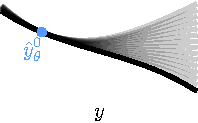
\includegraphics[width=2in]{fig/imaml.pdf}
\caption{Illustration of the penalty used in the Implicit MAML
  by \citet{rajeswaran2019meta} in \cref{eq:iMAML}.
  The original loss $f(y; x)$ is shown in black for
  a fixed context $x$ and the lighter grey colors
  show the impact of varying $\lambda$.
  This shows that the quadratic term of the penalization eventually
  overtakes the original loss and makes an optimum appear
  close to $\hat y_\theta^0$}
\label{fig:imaml}
\end{figure}

A huge issue arising in semi-amortized models is that adapting
to long time horizons is computationally and memory inefficient
and even if it wasn't, causes exploding, vanishing, or
otherwise unstable gradients.
An active direction of research seeks to solve these issues by
solving a smaller, local problem with the semi-amortized model,
such as in \citet{chen2019modular,rajeswaran2019meta}.
Implicit differentiation is an alternative to unrolling through
the iterations of a semi-amortized model in settings where the
model is able to successfully solve an optimization problem.

This section briefly summarizes \emph{Implicit MAML} (iMAML) by \citet{rajeswaran2019meta},
which notably brings this insight to MAML.
MAML methods usually only take a few gradient steps and
are usually not enough to globally solve \cref{eq:opt},
especially at the beginning of training.
\citet{rajeswaran2019meta} observe that adding a penalty
to the objective around the initial iterate
$\hat y^0_\theta$ makes it easy for the model to
\emph{globally} (!) solve the problem
\begin{equation}
  \label{eq:iMAML}
  \hat y_\theta(x) \in \argmin_y f(y; x) + \frac{\lambda}{2}\|y-\hat y^0_\theta\|_2^2,
\end{equation}
where the parameter $\lambda$ encourages the
solution to stay close to some initial iterate.
\Cref{fig:imaml} visualizes a function $f(y; x)$
in black and add penalties in grey with
$\lambda\in[0,12]$ and see that a global
minimum is difficult to find without adding a penalty
around the initial iterate.
This global solution can then be implicitly differentiated to obtain
a derivative of the loss with respect to the model's parameters
\emph{without} needing to unroll, as it requires
significantly less computational and memory resources.
\citet{huszar2019imaml} further analyzes and discuses iMAML.
They compare it to a Bayesian approach and observe that the insights
from iMAML can transfer from gradient-based meta-learning to
other amortized optimization settings.

\textbf{Warning.} Implicit differentiation is only useful
when optimization problems are exactly solved and satisfy
the conditions of the implicit function theorem in \cref{thm:dini}.
This is why \citet{rajeswaran2019meta} needed to add a penalty
to MAML's inner optimization problem in \cref{eq:iMAML} to
make the problem exactly solvable.
While they showed that this works and results in significant
improvements for differentiation, it comes at the expense of
changing the objective to penalize the distance from the
previous iterate.
In other words, iMAML modifies MAML's semi-amortized model
and in general is not helpful for estimating the derivative
through the original formulation of MAML.
Furthermore, computing the implicit derivative by
solving the linear system with the Jacobian
in \cref{eq:implicit-derivative} may be memory and
compute expensive to form and estimate exactly.
In practice, some methods such as \citet{bai2019deep}
successfully use indirect and approximation methods
to solve for the system in \cref{eq:implicit-derivative}.

\subsection{Learning with zeroth-order methods
  and RL}
\label{sec:learning:rl}

\begin{figure}[t]
\centering
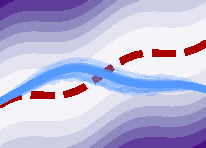
\includegraphics[width=2in]{fig/learning-rl.pdf}
\caption{Illustration of perturbing $\hat y_\theta$.
  A zeroth-order optimizers may make perturbations
  like this to search for an improved parameterization
}
\label{fig:perturbing}
\end{figure}

Computing the derivatives to learn $\hat y_\theta$ with a
first-order method may be impossible or unstable.
These problems typically arise when learning components
of the model that are truly non-differentiable, or
when attempting to unroll a semi-amortized model for
a lot of steps.
In these settings, research has successfully explored
other optimizers that do \emph{not} need the gradient information.
These methods often consider settings that improve
an objective-based loss with small local perturbations
rather than differentiation.
\Cref{fig:perturbing} illustrates that most of these
methods can be interpreted as locally perturbing the
model's prediction and updating the parameters to
move towards the best perturbations.

\subsubsection{Reinforcement learning}
\citet{li2016learning,li2017learning,ichnowski2021accelerating} view their
semi-amortized models as a Markov decision process (MDP)
that they solve with reinforcement learning.
The MDP interpretation uses the insight
that the iterations $x^i$ are the actions,
the context and previous iterations or losses are typically the states,
the associated losses $\gL(x^i)$ are the rewards,
and $\hat y_\theta^i(x)$ is a (deterministic) policy,
and transitions given by updating the current iterate,
either with a quantity defined by the policy or by running
one or more iterations from an existing optimizer.
Once this viewpoint is taken, then the optimal amortized model
can be found by using standard reinforcement learning methods,
\eg \citet{li2016learning,li2017learning} uses Guided Policy Search \citep{levine2013guided}
and \citet{ichnowski2021accelerating} uses TD3 \citep{fujimoto2018td3}.
The notation $\gL^{\rm RL}$ indicates that a loss is optimized with reinforcement learning,
typically on the objective-based loss.

\subsubsection{Loss smoothing and optimization with zeroth-order methods}
\label{sec:smooth}

Objective-based losses can have a high-frequency
structure with many poor local minimum.
\citet{metz2019understanding} overcome this by smoothing
the loss with a Gaussian over the \emph{parameter} space, \ie,
\begin{equation}
  \gL^{\rm smooth}(\hat y_\theta)\defeq \E_{\epsilon\sim\gN(0,\sigma^2 I)}\left[\gL(\hat y_{\theta+\epsilon})\right],
  \label{eq:smooth-loss}
\end{equation}
where $\sigma^2$ is a fixed variance.
\Cref{fig:smooth-loss} illustrates a loss function $\gL$ in
black and shows smoothed versions in color.
They consider learning the loss with reparameterization
gradients and zeroth-order evolutionary methods.
\citet{merchant2021learn2hop} further
build upon this for learned optimization in
atomic structural optimization
and study 1) clipping the values of the gradient estimator,
and 2) parameter optimization with genetic algorithms.

\begin{figure}[t]
\centering
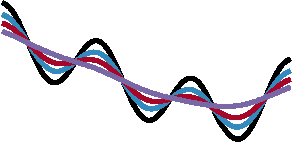
\includegraphics[width=2.1in]{fig/smoothed-loss.pdf}
\caption{Gaussian smoothing of a loss using \cref{eq:smooth-loss}.
  The colors show different values of the variance $\sigma^2$
  of the Gaussian. Selecting a high enough variance results in
  smoothing out most of the suboptimal minima.}
\label{fig:smooth-loss}
\end{figure}

\begin{remark}
  While smoothing can help reduce suboptimal local
  minima, it may also undesirably change the
  location of the global minimum.
  One potential solution to this is to decay
  the smoothing throughout training, as done
  in \citet[Appendix~A.1]{amos2021model}.
\end{remark}

\textbf{Connection to smoothing in reinforcement learning.}
The Gaussian smoothing of the objective $\gL$ in \cref{eq:smooth-loss}
is conceptually similar to Gaussian smoothing of the
objective in reinforcement learning, \ie the $-Q$-value,
by a Gaussian policy. This happens in
\cref{eq:Q-opt-sto-exp} and is further discussed
in \cref{sec:apps:ctrl}.
The policy's variance is typically controlled to match a
target entropy \citet{haarnoja2018soft} and the learning
typically starts with a high variance so the policy has a
broad view of the objective landscape and is then able to focus in
on a optimal region of the value distribution.
\citet{amos2021model} uses a fixed entropy decay schedule to
explicitly control this behavior.
In contrast, \citet{metz2019understanding,merchant2021learn2hop}
do not turn the loss into a distribution and more directly
smooth the loss with a Gaussian with a fixed variance $\sigma^2$
that is not optimized over.

\section{Extensions}
\label{sec:extensions}

I have intentionally scoped \cref{def:amor} to optimization problems
over \emph{deterministic, unconstrained, finite-dimensional, Euclidean}
domains $\gY$ where the context distribution $p(x)$
remains \emph{fixed} the
entire training time to provide a simple mental model that
allows us to focus on the core amortization principles
that consistently show up between applications.
This section cover extensions from this setting that may come up in practice.

\subsection{Extensions of the domain $\gY$}
\label{sec:extensions:domain}
\subsubsection{Deterministic $\rightarrow$ stochastic optimization}
\label{sec:extensions:sto}
A crucial extension is from optimization over deterministic vector
spaces $\gY$ to \emph{stochastic optimization}
where $\gY$ represents a space of distributions,
turning $y\in\gY$ from a vector in Euclidean space
into a distribution.
This comes up in \cref{sec:apps:ctrl} for control,
for example..

\textbf{Transforming parameterized stochastic problems
  back into deterministic ones.}
This portion will mostly focus on settings that
optimize over the parametric distributions.
This may arise in stochastic domains for variational inference in
\cref{sec:apps:avi} and stochastic control in \cref{sec:apps:ctrl}.
These settings optimize over a constrained parametric family
of distributions parameterized by some $\lambda$, for example
over a multivariate normal $\gN(\mu, \Sigma)$ parameterized
by $\lambda\defeq (\mu, \Sigma)$.
Here, problems can be transformed back to \cref{eq:opt} by
optimizing over the parameters with
\begin{equation}
  \lambda^\star(x) \in \argmin_{\lambda} f(\lambda; x),
  \label{eq:normal-opt}
\end{equation}
where $\lambda$ induces a distribution that the
objective $f$ may use.
When $\lambda$ is not an unconstrained real space, the
differentiable projections discussed in \cref{sec:constraints}
could be used to transform $\lambda$ back into this form for amortization.

\begin{figure}[t]
% \vspace{-2mm}
\centering
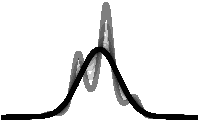
\includegraphics[width=2.3in]{fig/maxent.pdf}
\caption{
  The Gaussian distribution can be characterized as the result of
  the optimization problem in \cref{eq:maxent}:
  constrained to the space of continuous distributions with
  a given mean and variance, the Gaussian distribution has
  the maximum entropy in comparison to every other distribution.
  This example parameterizes a non-Gaussian density (shown in grey)
  and optimizes over it using gradient steps of \cref{eq:maxent},
  eventually converging to a Gaussian.
  An animated version is available
  \href{https://github.com/facebookresearch/amortized-optimization-tutorial/blob/main/paper/fig/maxent.gif}{in the repository associated with this tutorial}.
  While the Gaussian is the known closed-form solution to
  this optimization problem and analytically known,
  more general optimization problems over densities
  without known solutions can also be amortized.
}
% \vspace{-2mm}
\end{figure}
\textbf{Optimizing over distributions and densities.}
More general stochastic optimization settings involve optimizing over
spaces representing distributions, such as the functional space
of all continuous densities.
Many standard probability distributions can be obtained and
characterized as the solution to a maximum entropy
optimization problem and is explored, \eg, in
\citet[Ch.~12]{cover2006elements},
\citet[p.~47]{guiasu1985principle}, and
\citet[\S6.2]{pennec2006intrinsic}.
For example, a Gaussian distribution $\gN(\mu, \Sigma)$
solves the following constrained maximum entropy
optimization problem over the space of continuous densities $\gP$:
\begin{equation}
  p^\star(\mu, \Sigma)\in \argmax_{p\in\gP} \HH_p[X]\; \subjectto\; \E_p[X] = \mu\; {\rm and}\; \Var_p[X] = \Sigma,
  \label{eq:maxent}
\end{equation}
where $\HH_p[X]\defeq -\int p(x)\log p(x){\rm d}x$ is the \emph{differential entropy}
and the constraints are on the mean $\E_p[X]$ and covariance $\Var_p[X]$.
\citet[Theorem~8.6.5 and Example~12.2.8]{cover2006elements} prove that the closed-form solution
of $p^\star$ is the Gaussian density.
This Gaussian setting therefore does not need amortization as the
closed-form solution is known and easily computed, but
more general optimization problems over densities do not necessarily
have closed-form solutions and could benefit from amortization.
While this tutorial does not study amortizing these problems, in some cases it may
be possible to again transform them back into deterministic optimization problems
over Euclidean space for amortization by approximating the density $g_\theta$
with an expressive family of densities parameterized by $\theta$.

\subsubsection{Unconstrained $\rightarrow$ constrained optimization}
\label{sec:constraints}
Amortized constrained optimization problems may naturally arise, for example
in the convex optimization settings in \cref{sec:apps:convex}
and for optimization over the sphere in \cref{sec:impl:sphere}.
Constrained optimization problems for amortization can often be represented as
an extension of \cref{eq:opt} with
\begin{equation}
  y^\star(x) \in \argmin_{y\in\gC} f(y; x),
  \label{eq:opt-constrained}
\end{equation}
where the constraints $\gC$ may also depend on the context $x$.
\Cref{rmk:optimality-loss} suggests one way of amortizing
\cref{eq:opt-constrained} by amortizing the objective-based loss
associated with the optimality conditions of the constrained problem.
A budding research area studies how to more generally include
constraints into the formulation.
\citet{baker2019learning,dong2020smart,zamzam2020learning,pan2020deepopf}
learn to warm-start for optimal power flow.
\citet{misra2021learning} learn active sets for constrained optimization.
\citet{krivachy2020fast} solves constrained feasibility semi-definite programs
with a fully-amortized neural network model using an
objective-based loss.
\citet{donti2021dc3} learns a fully-amortized model and optimizes an
objective-based loss with additional completion and correction terms
to ensure the prediction satisfies the constraints of the original problem.


\begin{figure}[t]
  \centering
  \begin{tikzpicture}[every path/.style={thick}]
    \path[fill=lightpurple!20] (0,0) coordinate(p1) -- ++(20:2) coordinate(p2) -- ++(-55:2.5)
    coordinate(p3) -- ++(-120:2.) coordinate(p4) --  ++(160:2.5) coordinate(p5);
    \node at (barycentric cs:p1=1,p2=1,p3=1,p4=1,p5=1) {$\gC$};
    \foreach \X [count=\Y] in {2,...,6} {
      \ifnum\X=6
      \path (p\Y) -- (p1) coordinate[pos=0.](a\Y) coordinate[pos=1.](a1)
      coordinate[pos=0.5](m1);
      \draw (a\Y) -- (a1);
      \else
      \path (p\Y) -- (p\X) coordinate[pos=0.](a\Y) coordinate[pos=1.](a\X)
      coordinate[pos=0.5](m\X);
      \draw (a\Y) -- (a\X);
      \fi}
    \draw[dashed] (m3) -- ($ (m3)!1.2cm!90:(p3) $) node[pos=1.2]{$x$}; %node[pos=-.3]{$\pi_\gC(x)$};
    \filldraw[black] (m3) circle(2pt);
    \filldraw[black] ($ (m3)!1.2cm!90:(p3) $) circle(2pt);
    \node[xshift=1pt,anchor=west] at (m3) {$\pi_\gC(x)$};
  \end{tikzpicture}
  \label{fig:projection}
  \caption{Illustration of \cref{def:proj} showing
    a Euclidean projection $\pi_\gC(x)$ of a point $x$
    onto a set $\gC$.}
\end{figure}


\textbf{Differentiable projections.}
When the constraints are relatively simple, a differentiable projection
can transform a constrained optimization problem into an unconstrained one,
\eg, in reinforcement learning constrained action spaces can be transformed
from the box $[-1,1]^n$ to the reals $\R^n$ by using
the $\tanh$ to project from $\R^n$ to $[-1,1]^n$.
\Cref{sec:impl:sphere} also uses a differentiable projection from $\R^n$
onto the sphere $\gS^{n-1}$.
These are illustrated in \cref{fig:projection} and defined as:
\begin{definition}
  A \emph{projection} from $\R^n$ onto a set $\gC\subseteq \R^n$ is
  \begin{equation}
    \pi_\gC: \R^n\rightarrow \gC \qquad \pi_\gC(x) \in \argmin_{y\in\gC} D(x, y) + \Omega(y),
    \label{eq:proj}
  \end{equation}
  where $D: \R^n\times\R^n\rightarrow \R$ is a distance and $\Omega:\R^n\rightarrow \R$ is
  a regularizer that can ensure invertibility or help spread $\R^n$ more uniformly throughout $\gC$.
  A \emph{(sub)differentiable projection} has (sub)derivatives $\nabla_x \pi_\gC(x)$.
  I sometimes omit the dependence of $\pi$ on the choice of $D$, $\Omega$, and $\gC$
  when they are given by the surrounding context.
  \label{def:proj}
\end{definition}

\textbf{Lack of idempotency.} In linear algebra, a projection is defined to
be \emph{idempotent}, \ie applying the projection twice gives the same result
so that $\pi\circ \pi=\pi$.
Unfortunately, projections as defined in \cref{def:proj},
such as Bregman projections, are \emph{not} idempotent in general
and often $\pi_\gC\circ \pi_\gC\neq \pi_\gC$
as the regularizer $\Omega$ may cause points that are already on $\gC$
to move to a different position on $\gC$.

\textbf{Differentiable projections for constrained amortization.}
These can be used to cast \Cref{eq:opt-constrained} as the unconstrained
problem \cref{eq:opt} by composing the objective with a projection
$f\circ \pi_\gC$.
(Sub)differentiable projections enable gradient-based learning through the projection
and is the most easily attainable when the projection has an explicit closed-form solution.
For intuition, the ReLU, sigmoid, and softargmax can be interpreted as
differentiable projections that solve convex optimization problems
in the form of \cref{eq:proj}.
\citet[\S2.4.4]{amos2019differentiable} further discusses these
and proves them using the KKT conditions:
\begin{itemize}
\item The standard Euclidean projection onto the
  \emph{non-negative orthant} $\R^n_+$ is defined by
  \begin{equation}
    \pi(x) \in \argmin_y \;\; \frac{1}{2}\|x-y\|_2^2 \;\; \st \;\; y\geq 0,
    \label{eq:relu-proj}
  \end{equation}
  and has a closed-form solution given by the
  ReLU, \ie $\pi(x) \defeq \max\{0, x\}$.
\item The interior of the \emph{unit hypercube} $[0,1]^n$ can
  be projected onto with the entropy-regularized
  optimization problem
  \begin{equation}
    \pi(x) \in \argmin_{0<y<1} \;\; -x^\top y -H_b(y),
    \label{eq:sigmoid-proj}
  \end{equation}
  where
  \begin{equation}
  H_b(y) = \defeq \left(\sum_i y_i\log y_i + (1-y_i)\log (1-y_i)\right)
  \end{equation}
  is the
  binary entropy function.
  \Cref{eq:sigmoid-proj} has a closed-form solution given by
  the \emph{sigmoid} or \emph{logistic} function,
  \ie $\pi(x) \defeq (1+e^{-x})^{-1}$.
\item The interior of the $(n-1)$-\emph{simplex} defined by
  \begin{equation}
    \Delta_{n-1}\defeq\{p\in\R^n\; \vert\; 1^\top p = 1 \; \; {\rm and} \;\; p \geq 0 \}
    \label{eq:simplex}
  \end{equation}
  can be projected onto with the entropy-regularized
  optimization problem
  \begin{equation}
    \pi(x) \in \argmin_{0<y<1} \;\; -x^\top y - H(y) \;\; \st\;\; 1^\top y = 1
    \label{eq:simplex-proj}
  \end{equation}
  where $H(y) \defeq -\sum_i y_i \log y_i$ is the entropy function.
  \Cref{eq:simplex-proj} has a closed-form solution given by
  the \emph{softargmax}, \ie $\pi(x)_j = e^{x_j} / \sum_i e^{x_i}$,
  which is historically referred to as the \emph{softmax}.
\end{itemize}

\begin{figure}[t]
  \centering
  \begin{tikzpicture}[every path/.style={thick}]
    \path[fill=lightpurple!20]
      (0,0) arc (-170:-10:1.5cm and 0.4cm)coordinate[pos=0]
      -- (0,0) arc (170:10:1.5cm and 0.4cm)coordinate;
    \draw (0,0) arc (-170:-10:1.5cm and 0.4cm)coordinate[pos=0] (a);
    \draw (0,0) arc (170:10:1.5cm and 0.4cm)coordinate (b);
    \draw (a) -- ([yshift=-3cm]$(a)!0.5!(b)$) -- (b);
  \end{tikzpicture}
  \label{fig:lorentz-cone}
  \caption{Illustration of the second-order cone in \cref{eq:lorentz-cone}.}
\end{figure}


This section goes beyond these to differentiable projections onto
\emph{convex cones}. These can also be softened or regularized
to help with continuity when composed with learning and
amortization methods.
\citet{ali2017semismooth,busseti2019solution} discuss
differentiating the standard Euclidean projections
onto these, including:
\begin{itemize}
\item
  The \emph{second-order, Lorentz, or ice cream cone}
  defined by
  \begin{equation}
    \gK_{\rm soc}\defeq\{(x,y)\in\R^{m-1}\times\R : \|x\|_2\leq y\},
    \label{eq:lorentz-cone}
  \end{equation}
  which is illustrated in \cref{fig:lorentz-cone}.
  The standard Euclidean projection is given in closed form as
  \begin{equation}
    \pi(x, y) \defeq
    \begin{cases}
      0 & \|x\|_2 \leq -y \\
      (x,y) & \|x\|_2 \leq y \\
      \frac{1}{2} (1 + \frac{y}{\|x\|_2}) (x, \|x\|_2) & \textrm{otherwise}.
    \end{cases}
  \end{equation}
  and can be explicitly differentiated.
\item The \emph{positive semidefinite cone} $\gS^m_+$ of the
  space of $m\times m$ positive semidefinite matrices.
  The Euclidean projection is obtained in closed-form
  by projecting the eigenvalues to be non-negative with
  $\pi(X)\defeq\sum_i\max\{\lambda_i, 0\}q_iq_i^\top$,
  where the eigenvalue decomposition of $X$ is given by
  $X=\sum_i\lambda_iq_iq_i^\top$.
  The derivative can be computed by differentiating
  through the eigenvalue decomposition and projection
  of the eigenvalues.
\item The \emph{exponential cone} is given by
  \begin{equation}
  \begin{aligned}
    \gK_{\rm exp} = & \{(x,y,z) : x\in\R, y>0, z\geq y\exp(x/y)\} \\
    & \cup \{(x,0,z): x\leq0, z\geq 0\}.
  \end{aligned}
  \label{eq:exp-cone}
  \end{equation}
  The standard Euclidean projection onto this does
  \emph{not} have a known closed-form solution
  but can be computed using a Newton method
  as discussed in
  \citet[\S6.3.4]{parikh2014proximal}.
  \citet{ali2017semismooth} differentiate through
  this projection using implicit differentiation
  of the KKT system.
\end{itemize}

\noindent Other uses of projections in machine learning include:
\begin{itemize}
\item \citet{adams2011ranking,santa2017deeppermnet,mena2018learning}
  project onto the \emph{Birkhoff polytope} of
  \emph{doubly stochastic} matrices with row and
  column sums of 1, \ie
  \begin{equation}
    \label{eq:birkhoff}
    \gB_m\defeq \{X\in\R^{m\times m}: X1=X^\top1=1\}.
  \end{equation}
\item \citet{amos2019limited} project onto the capped
  simplex for a differentiable top-$k$ layer.
\item \citet{blondel2019structured} perform structure
  prediction and learning methods building on Fenchel-Young losses
  \citep{blondel2020learning} and use projections onto the
  simplex, unit cube, knapsack polytope, Birkhoff polytope,
  permutahedron, and order simplex.
\end{itemize}

In many of these, the projections have explicit closed-form
solutions that make it easy to compute and differentiate
through the projections for learning.
When a closed-form solution to the projection is not available to
the project, but the projection can be numerically computed,
projections can often still be differentiated through using
implicit differentiation.

\subsubsection{Euclidean $\rightarrow$ non-Euclidean optimization}
\emph{Manifold optimization} \citep{absil2009optimization,hu2019brief}
over non-Euclidean spaces is a thriving topic in optimization
as these problems arise frequently over complex geometries in nature.
One form of manifold optimization takes $\gY$ to be a Riemannian
manifold rather than a real-valued spaced.
This area of research has studied acceleration methods,
\citep{duruisseaux2022accelerated}, but less exploration
has been done on amortized optimization.
\Cref{sec:impl:sphere} discusses amortizing a simple
constrained spherical optimization problem that can be
transformed into an unconstrained Euclidean optimization
problem by using projections from ambient Euclidean space.
When this is not possible, a budding area of research investigates
more directly including the manifold structure into the
amortization process. \citet{gao2020learning} amortize optimization
problems over SPD spaces.

\subsection{Extensions of the model $\hat y_\theta$}
Finding the best model for an amortized optimization setup
is an active research topic in many areas.
While the tutorial is mostly scoped to differentiable
parametric models that are end-to-end learned,
variations and extensions can be considered.

\subsubsection{Symbolic models: uncovering human-interpretable update rules}
A huge issue of neural-network based amortization models
is that they are uninterpretable and it is often impossible
for us as humans to learn any new insights about the optimization
problems being modeled, \eg how to better-solve them.
Symbolic models are one potential answer to this that attempt
to search over a symbolic space that is much closer to the
operations that humans would use to implement update rules for
an optimization solver.
Early studies of these methods include
\citet{bengio1994use,runarsson2000evolution}.
\citet{bello2017neural} significantly advances this direction
by posing the learned optimizer as a reinforcement learning problem
where the actions produce the operations underlying the update rules.
They show how existing methods can be symbolically implemented
using this formulation, and learn better update rules for
classification and machine translation tasks.
Symbolic methods are further studied and scaled in
\citet{real2020automl,zheng2022symbolic}.
\citet{maheswaranathan2021reverse} reverse engineer learned
optimizers and show that they have learned interpretable behavior,
including momentum, gradient clipping, learning rate schedules,
and learning rate adaptation.

This direction of work challenges the best accelerated and adaptive
gradient-based optimizers that are used for machine learning.
Nesterov acceleration \citep{nesterov1983method} has a provably
optimal convergence rate among first-order methods for solving
convex optimization problems, but unfortunately breaks down
in the non-convex setting.
This has led to a stream of variations of acceleration methods
for non-convex problems that come up in machine learning,
such as \citet{duchi2011adaptive,zeiler2012adadelta,kingma2014adam},
that typically add components that adapt the update rules to
how much the objective is moving in each dimension.
None of these algorithms are theoretically or provably the
best in non-convex settings, and is often empirically validated
depending on the domain.
Using amortized optimization with a symbolic model to search
the design space of optimizers can result is significantly
better optimizers and insights into the optimization problems
being solved, especially when this is done on new classes
of problems beyond the parameter learning problems typically
considered in machine learning settings.

\subsection{Uncertainty-aware and Bayesian optimization}
An active research direction combines \emph{uncertainty} estimation
and amortized optimization:

\textbf{Amortization for Bayesian optimization.}
\citet{chen2017learning} propose to use an RNN-based
  amortization in Bayesian optimization settings that
  predict the optimal solution to commonly used
  acquisition functions such as the expected improvement
  and observed improvement.
  This is powerful as optimizing the acquisition function
  is often a computational bottleneck.
\citet{swersky2020amortized} consider amortized
  Bayesian optimization in discrete spaces and show
  applications to protein sequence design.
\citet{ravi2018amortized} propose amortized
  Bayesian meta-learning for meta-learning with uncertainty
  estimation over the posterior and show applications to
  contextual bandits and few-shot learning.

\textbf{Bayesian methods for amortization.}
\citet{you2022bayesian} investigate \emph{optimizer uncertainty}
or \emph{Bayesian learning to optimize}.
This setting explores the uncertainty that an optimizer,
\eg the amortization model, is the best optimizer for
the problem.


\subsection{Settings with additional learnable contexts $\varphi$}
The amortization model is often a component within a larger system
with other learnable parameters that are being optimized over.
This is done in, for example, 1) variational autoencoders
where the ELBO also depends on the decoder's parameters
that are also being optimized over,
2) deep equilibrium models where the fixed point
is parameterized and optimized over, and
3) reinforcement learning where the value estimate is
also parameterized and learned over.

These dependencies can be captured by writing an explicit
dependence of the context distribution and objective
on an additional parameter $\varphi$, \ie as $p(x; \varphi)$
and $f(y; x, \varphi)$.
$\varphi$ can be learned with a higher-level optimization
process with a loss $\ell$ defined on the \emph{solutions}.
This could take the form of the bi-level problem
\begin{equation}
  \argmin_{\varphi} \E_{x\sim p(x)} \ell(y^\star(x, \varphi); x, \varphi)\;
  \subjectto\; y^\star(x, \varphi)\in\argmin_y f(y; x, \varphi)
\label{eq:learn-context}
\end{equation}
where $y^\star(x, \varphi)$ can be replaced with an approximation
by a learned amortization model $\hat y_\theta \approx y^\star$.
The parameters $\varphi$ in \cref{eq:learn-context} can
often by end-to-end learned \emph{through the solution} of
\cref{eq:opt} to update the influence that $\varphi$
has on the solutions.
The next section turns to methods that show how to differentiate
through the value $f(y^\star(x, \varphi); x, \varphi)$ and solution
$y^\star(x, \varphi)$ to enable gradient-based learning of
$\varphi$ in \cref{eq:learn-context}.

\subsubsection{Learning $\varphi$ by differentiating
  the objective value $f(y^\star(x, \varphi); x, \varphi)$}
Methods can end-to-end learn through the \emph{optimal objective value}
$f(y^\star(x, \varphi); x, \varphi)$ to update parameters $\varphi$
that show up in the context --- \ie by taking $\ell=f$ in \cref{eq:learn-context}.
For example, variational autoencoders differentiate through
the objective value, \ie the best approximation to the ELBO,
to optimize the data log-likelihood of a parameterized
decoder $\log p(x\mid z; \varphi)$.
The theory around this is rooted in the optimization
community's studies of \emph{envelope theorems},
which describe settings where the minimum value
can be differentiated by just differentiating
the objective.
\emph{Danskin's envelope theorem} \citep{danskin1966theory}
in convex settings is one of the earliest and has been
extended into more general settings, \eg, in
\citep[Prop. A.22]{bertsekas1971control}
and \cite{carter2001foundations,milgrom2002envelope,bonnans2013perturbation}.
In the unconstrained and non-convex \cref{eq:opt},
the envelope theorem gives
\begin{equation}
  \nabla_\varphi \min_y f(y; x, \bar\varphi) = \nabla_\varphi f(y^\star(x, \bar\varphi); x, \bar\varphi)
  \label{eq:envelope}
\end{equation}
at a point $\bar\varphi$ under mild assumptions, showing
that differentiating through the $\min$ operation is equivalent to differentiating
through just the objective at the optimal solution $y^\star(x, \varphi)$.

\subsubsection{Learning $\varphi$ by differentiating the solution $y^\star(x, \varphi)$}
In addition to differentiating through the objective value, the solution
$y^\star(x, \varphi)$ can be implicitly differentiated.
The derivative $\D_\varphi y^\star(x, \varphi)$ is referred to
as the \emph{adjoint derivative}, and it is often used for
end-to-end learning
\citep{domke2012generic,gould2016differentiating,amos2017optnet,barratt2018differentiability,amos2019differentiable,agrawal2019differentiable,bai2019deep,bai2020multiscale}
and perturbation and sensitivity analysis
\citep{bank1982non,fiacco1990sensitivity,shapiro2003sensitivity,klatte2006nonsmooth,bonnans2013perturbation,still2018lectures,fiacco2020mathematical}.

Computing the adjoint derivative $\D_\varphi y^\star(x, \varphi)$ is more involved
than the value derivative using the envelope theorem
in \cref{eq:envelope} as more components of $y^\star(x)$
can change as $x$ moves infinitesimally.
An explicit closed-form solution to $y^\star(x)$ is
not available in most cases, which means that standard
methods for explicitly computing the derivative through
this computation may not work well or may break down.
For example, an optimizer to compute $y^\star(x)$ may be
explicitly unrolled through, but this may be
unstable and extremely memory- and compute-intensive
to track all of the iterations.
The adjoint derivative is typically computed with implicit
differentiation by seeing $y^\star(x)$ as an \emph{implicit}
function of $x$.
This uses the implicit function theorem,
which is originally from \citet{dini1878analisi},
and is presented in \citet[Theorem 1B.1]{dontchev2009implicit} as:
\begin{theorem}[Dini's implicit function theorem]
  \label{thm:dini}
  Let the roots of $g(y; \varphi)$ define an implicit
  mapping $Y^\star(\varphi)$ given by $Y^\star(\varphi)\defeq\{y \mid g(y;\varphi)=0\}$,
  where $\varphi\in\R^m$, $y\in\R^n$, and
  $g: \R^n\times\R^m\rightarrow\R^n$.
  Let $g$ be continuously differentiable in a neighborhood of $(\bar y, \bar \varphi)$
  such that $g(\bar y; \bar \varphi)=0$, and let the Jacobian of $g$
  with respect to $y$ at $(\bar y, \bar \varphi)$,
  \ie $\D_y g(\bar y; \bar \varphi)$, be non-singular.
  Then $Y^\star$ has a single-valued localization $y^\star$
  around $\bar \varphi$ for $\bar y$ which is continuously differentiable
  in a neighborhood $Q$ of $\bar \varphi$ with Jacobian satisfying
  \begin{equation}
    \D_\varphi y^\star(\tilde \varphi) = -\D_y^{-1} g(y^\star(\tilde \varphi); \tilde \varphi) \D_\varphi g(y^\star(\tilde \varphi); \tilde \varphi)
    \qquad \mathrm{for\ every}\; \tilde \varphi\in Q.
    \label{eq:implicit-derivative}
  \end{equation}
\end{theorem}

The adjoint derivative $D_\varphi y^\star(\varphi)$ can be computed
by seeing $y^\star$ as the root of an implicit
function $g(y;x,\varphi)$, which needs to be selected to
make the solution equivalent to the solution of \cref{eq:opt}.
Typically $g(y;x,\varphi)$ is an optimality system of
the optimization problem, \eg the KKT system
for constrained convex optimization problems.
For the unconstrained problem here,
the first-order optimality of
the objective $g(y;x, \varphi) \defeq \nabla_y f(y; x, \varphi)$
can be used with \cref{thm:dini} to compute
$\D_\varphi y^\star(x, \varphi)$.

%%% Local Variables:
%%% coding: utf-8
%%% mode: latex
%%% TeX-master: "../amor-nowplain.tex"
%%% LaTeX-biblatex-use-Biber: True
%%% End: